% !TEXroot=main.tex
\section{ROS}
{
	\subsection{Überblick}
	{
		Das sogenannte Robot Operating System, kurz ROS genannt, ist ein Open-Source Betriebssystem für Roboter, welches viele Tools und Software-Bibliotheken bietet. Die Entwicklung von ROS begann 2007 im Stanford Artificial Intelligence Laboratory. Ab 2009 wurde ROS im Institut Willow Garage fortgeführt, bis ROS ab 2012 von der OSRF (Open Source Robotic Foundation) unterstützt wird. Seit der Veröffentlichung von ROS gibt es regelmäßig Updates und neuere Versionen von ROS, welche hauptsächlich mit Betriebssystem Linux, aber auch Windows oder MacOS kompatibel sind. 
		
		Die grundsätzliche Idee von ROS ist, alle Vorteile von vergleichbaren Produkten zu vereinen, während die Nachteile der jeweiligen Produkte behoben werden. Die Hauptbestandteile von ROS sind: Hardwareabstraktion, Gerätetreiber, Nachrichtenaustausch zwischen Programmen und Programmteilen und die Paketverwaltung. Alle diese Bestandteile sorgen dafür, dass der Roboter einfacher auf Daten zugreifen kann. Es handelt sich dabei um den aktuellen internationalen Standard, welcher auf den meisten Systemen einwandfrei läuft und dabei wenig Leistung beansprucht. Ein Gerätetreiber ist ein Programm, welches die Interaktion mit angeschlossenen, eingebauten oder virtuellen Geräten steuert. Beim Nachrichtenaustausch werden Nachrichten zum Empfänger versendet, bei welchen es sich um Signale oder Datenpakete handeln kann. Die Paketverwaltung hilft bei der Verwaltung von Software, die in Form von Programmpaketen vorliegt. Ein weiteres Ziel von ROS ist, oft wiederverwendbare Funktionen zugänglich zu machen. 
		
	}

	\subsection{Aufbau}
	{ Programme werden in ROS als Pakete implementiert. Ein Paket besteht aus einer Manifestdatei, welche Metadaten (z.B. den Autor) über das Paket beinhaltet, sowie ausführbaren Skripten (Programmen). Pakete werden meist unabhängig voneinander entwickelt, können doch miteinander kommunizieren (siehe Datenaustausch). Pakete können (ähnlich zu Apps auf einem Handy) einzeln installiert bzw. deinstalliert werden, wobei einige Pakete andere benötigen, um zu funktionieren. Die Programme werden meist in den Programmiersprachen C++ oder Python geschrieben, welche beide die größte Integration in das ROS vorweisen.
	
	Der ROS-Core ist der Mittelpunkt des Betriebssystems. Dieses Programm steuert alle Vorgänge und sorgt dafür, dass Daten an korrekte Pakete weitergegeben werden, sowie vieles mehr. 
	
	Eine Grundkomponente von ROS sind sogenannte Nodes (Knotenpunkte), welche von Programmen initiiert werden können: Jede dieser Nodes hat eine gewisse Funktion (z.B. das ansteuern von Motoren). Diese Punkte sind des Weiteren austauschbar, sodass es für verschiedene Motorenmodelle beispielsweise andere Nodes gibt, welche jedoch alle die gleiche Funktion erfüllen, nämlich das ansteuern der Motoren.
	}

	\subsection{Datenaustausch}
	{
		Der Austausch von Daten kann sich als Graph vorgestellt werden. Jeder Knotenpunkt kann Daten aussenden oder empfangen. Der Datentyp, welcher ausgetauscht wird, kann beliebig bestimmt werden, jedoch beruht alles auf vier Grundtypen.
		\begin{enumerate}
			\item Ganzzahlen (Integer)
			\item Kommazahlen (Float)
			\item Zeichen (Char)
			\item Ja/Nein (Boolean)
		\end{enumerate}
		Basierend auf diesen Grundtypen können neue Datentypen gebaut werden. So kann man beispielsweise sagen, dass der Datentyp Auto
		\begin{enumerate}
			\item eine Kommazahl hat, welche den Füllstand beschreibt,
			\item eine ganze Zahl hat, welche die Anzahl an Passagieren beschreibt,
			\item ein aus mehreren Zeichen bestehendes Kennzeichen hat,
			\item einen Ja/Nein-Wert hat, welcher bestimmt, ob der Motor an ist,
		\end{enumerate}
		
		hat. Die Datenstruktur der ausgetauschten Daten wird Nachricht genannt. Nodes tauschen also Nachrichten untereinander aus. Jede Nachricht bekommt eine sogenannte Topic, was die Nachricht und deren Struktur eindeutig identifiziert. Ein Beispiel hierfür ist die \textit{cmd\textunderscore vel} Topic, welche Nachrichten des Types \textit{geometry\textunderscore msgs/Twist} weitergibt. Diese Daten geben Informationen über die aktuelle Begungsrichtung wieder. Zur vereinfachung zeige ich nur die Richtungen der Bewegung im 3D-Raum, nicht aber der Drehung, da diese für das Verständnis nicht notwendig ist. Die Struktur der Nachricht sieht daher (in gekürzter Fassung folgendermaßen aus:
		\newline
		
		linear:
		\begin{itemize}
			\item float64 x
			\item float64 y
			\item float64 z
		\end{itemize}
		
		\textit{float64} stellt in der Programmierung eine Kommazahl dar. Daraus folgt, dass diese Nachricht drei Zahlen für jede Richtung hat, woraus sich die Bewegungsrichtung des Roboters ergibt. Im Falle meiner NAvigation ist die z-Koordinate irrelevant, da der Roboter sich nicht nach oben/unten bewegt, sondern nur auf der 2 dimensionalen Ebene.
	}
	
	\subsubsection{Publisher-Subscriber}
	{
		Nodes sind von Programmen initiierte Knotenpunkte, auf welche das Programm ,welches sie initiiert hat, Zugriff hat. Über diese Punkte können Daten bereitgestellt werden, indem das Programm diese publiziert (Publisher). Dies kann man sich wie ein Forum darstellen, in welchem eine Person mit einem Megafon die Daten verkündet. Andere Nodes (Listener/Subscriber) können diesen Punkt nun abonnieren, was bedeutet, dass die Daten an sie weitergeleitet werden. Diese Listener-Nodes sind vergleichbar mit Personen, die das Forum betreten und daher alles hören, was der Redner (Publisher-Node) sagt. bei dieser Variante des Datenaustausches bestimmt der Publisher, wann Daten verbreitet werden. Mehrere Listener-Nodes können eine Publisher-Node abonnieren.
	}
	\subsubsection{Services}
	{ 
		Services bilden das Gegenstück zum Publisher-Subscriber-Modell. Hierbei stellt eine Node Aufgaben bereit, welche sie auf Anforderung erfüllt. Node A bietet beispielsweise an, die Lichter in einem Raum an bzw. auszuschalten. Node B kann in diesem Fall auf den Service "Ändere Lichtzustand" von Node A zugreifen, woraufhin Node A das Licht an bzw. ausschaltet. Ohne Aufruf führt Node A dies jedoch nicht durch. Dies zeigt, dass bei diesem Modell nicht, die Node, welche einen Service bereitstellt, den Zeitpunkt der Ausführung definiert, sondern ein anderer Punkt, welcher den Service aufruft.
	}

	\subsection{Visualisierung des Datenaustausches}
	{
		Der Datenaustausch zwischen verschiedenen Nodes kann mit Hilfe einfacher Tools visualisiert werden. Ein sehr wichtiges Tool ist \textit{rqt\textunderscore Graph}, welches alle Knoten und deren Zusammenhänge als Graphen anzeigt. Dabei werden Nodes als Punkte und deren Verbindungen als Linien angezeigt. Verbindungen werden mit dem Namen der Topic an Daten, die Übertrieben werden, beschriftet. Dies ist vereinfacht in Abbildung 1 dargestellt. Hierbei veröffentlicht die Node \textit{number\textunderscore publisher} Daten der Topic \textit{/number} an die Node \textit{number\textunderscore subscriber} (rechts), welche die linke Node abonniert hat.
		
		\begin{figure}
			\centering
			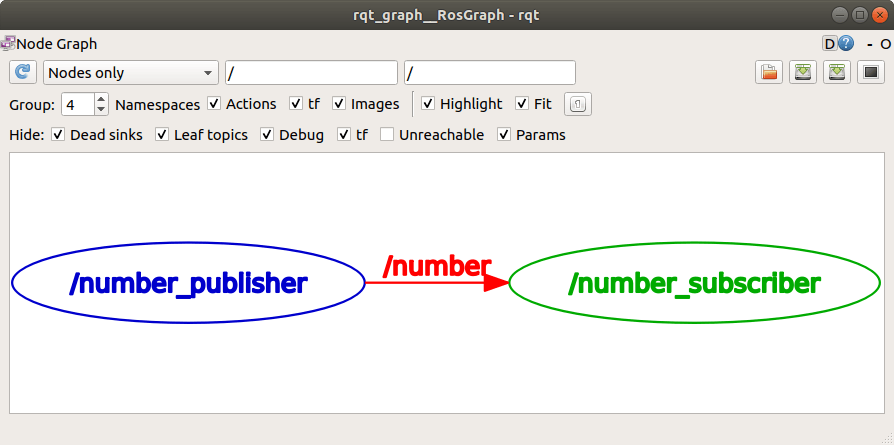
\includegraphics[height=5cm]{Bilder/rqt_graph_simplified.png}
			\caption{Ein vereinfachter Graph \\
			\parencite{rqtgraphsimplified1}} 
			\label{pic:rqt_graph_simplified}
		\end{figure}
	}

	\subsection{Drahtlose Übertragung}
	{ Wie bereits erwähnt, besitzt der Turtlebot einen Raspberry Pi. Dieser besitzt zwar für seine Größe vergleichsweise viel Leistung, jedoch wäre es natürlich vorteilhaft, die Rechenleistung eines herkömmlichen Desktop-PCs zu nutzen. Genau deshalb ermöglicht es das ROS, über mehrere Geräte hinweg zu kommunizieren. Das Herzstück bildet hierbei das ROS-Core Programm, welches alle Vorgänge innerhalb des Systems steuert. Dieses Programm muss auf einem der miteinander kommunizierenden Geräte aktiv sein. Mit Hilfe IP-Adressen \footnote{Ähnlich einer Adressanschrift: Zahlenkombination zur eindeutigen Identifikation eines Gerätes in einem Netzwerk} der Geräte kommunizieren die Teilnehmer untereinander in einem Netzwerk, als ob alle Pakete (Programme) auf einem Geräte ausgeführt werden würden. Dies ermöglicht das ausführen von Rechenintensiven Programmen auf einem Computer, während kleinere Programme, sowie der ROS-Core auf dem Turtlebot laufen. Das Gerät, auf welchem der Ros-Core läuft, wird auch ROS-Master genannt. Um beide Geräte zu verbinden, benötigt es nur wenige Einstellungen. Nachdem beide Geräte sich im gleichen Netzwerk befinden müssen die Parameter: \textbf{ROS\textunderscore IP} und \textbf{ROS\textunderscore Master \textunderscore URI} eingestellt werden. Ersterer beschreibt die IP-Adresse des Gerätes (für beide Geräte unterschiedlich) und letzterer Parameter beschreibt die IP-Adresse des ROS-Masters (für beide gleich, in meinem Fall ist es die Ip-Adresse des Turtlebot). Durch das ROS bauen beide Geräte eine Verbindung miteinander auf und kommunizieren miteinander.
	}
	
	\subsection{Simulation und Visualisierung}
	{
		Gazebo ist ein Open-Source-Programm \footnote{Frei zur Verfügung gestellt}, welches eine vollständige Simulation von Robotern, Umgebungen und Messungen ermöglicht. Robotermodelle können dazu modelliert werden, ebenso wie Umgebungen. Der Roboter kann sich daraufhin, wie in der realen Welt, bewegen und Messungen durchführen. Durch eine realistische Physik-Engine\footnote{Virtuelle Simulation physikalischer Kräfte} können Messungen wie in der echten Welt simuliert werden. D.h. der simulierte Roboter, in meinem Fall der Turtlebot, erhält Messdaten durch seinen Sensor, welche basierend auf der virtuellen Welt errechnet werden. Da ich einen größeren Teil meiner Arbeit von zuhause verrichtet habe, wurde dieses Programm oft genutzt, weshalb auch immer Bilder aus diesem Programm, anstelle von Bildern aus der echten Welt, gezeigt werden.
		
		Rviz ist ebenso ein Open-Source-Tool, welches es ermöglicht, Daten, ob gemessen oder errechnet, zu visualisieren. Dafür empfängt ROS Daten der Nodes und präsentiert diese auf geeigneter Weise. So kann beispielsweise die Momentane Bewegungsrichtung als Pfeil, Messdaten des LiDAR-Sensors als Punkte oder eine Errechnete Karte als Hintergrundbild angezeigt werden
		
		
	}
}